\documentclass[10pt,a4paper]{article}
\usepackage[margin=18mm]{geometry}
\usepackage[T1]{fontenc}
\usepackage{lmodern,graphicx,booktabs,hyperref,xcolor}
\hypersetup{colorlinks=true,urlcolor=blue}
\pagestyle{empty}
\setlength{\parindent}{0pt}
\setlength{\parskip}{6pt}
\begin{document}
{\LARGE Independent admission replay}\par
{\large Before expanding classical prime-field ECDLP targets}\par
23 November 2026. Native C/OpenSSL; local only; S3 excluded.

\textbf{Observed result.} The frozen checker returned all prescribed
classifications: 199 control rows and 12 recorded public targets across 6 full
prime-order domains. All 6 domains passed the recorded exceptional-class
screen. These are unsigned producer observations [pcc:unverified].

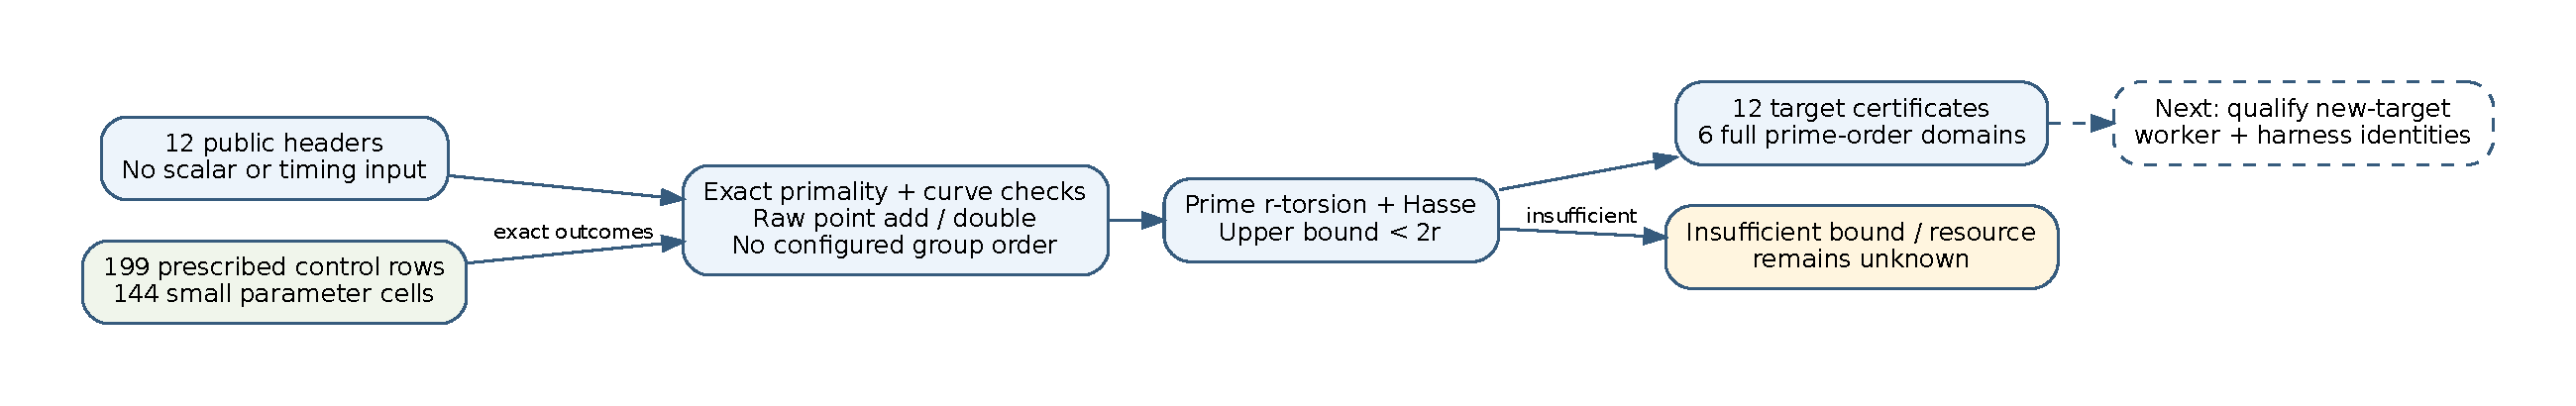
\includegraphics[width=\linewidth]{admission-figure.pdf}

\textbf{Method.} Public headers contain no recovered scalar or timing.
Exact trial division, canonical/on-curve checks and explicit point addition
and doubling precede the Hasse certificate. OpenSSL has no configured group
order or finite generator; the source never calls \texttt{EC\_POINT\_mul}.
This independently implements the existing Rust constructor method.

For nonzero prime $r$-torsion, Lagrange gives $r\mid N$. Hasse gives
$0<N\le p+1+\lfloor\sqrt{4p}\rfloor$. If that upper bound is below $2r$,
then $N=r$. This reuses established mathematics, not a new mechanism or a
full C/OpenSSL-to-Lean refinement. See
\href{https://www.secg.org/sec1-v2.pdf}{SEC1v2, section 3.1.1.2.1} and
\href{https://math.mit.edu/classes/18.783/2025/LectureNotes7.pdf}{Sutherland,
Lecture 7, Theorem 7.3 and section 7.4}.

\begin{center}
\begin{tabular}{lrp{100mm}}
\toprule
Control class & Rows & Required observation \\
\midrule
Square root & 1 & Both postconditions for every integer 0--65535 \\
Known composites & 3 & Reject with a nontrivial divisor \\
Small curve cells & 144 & Match direct enumeration and literal prime table \\
Literal cases & 2 & Anomaly flagged; singularity rejected \\
Domain mutants & 48 & Exact specified rejection cause \\
Oversized input & 1 & Unknown/resource with zero arithmetic work \\
Public targets & 12 & Prime full order and point certificate \\
\bottomrule
\end{tabular}
\end{center}

\textbf{Controls and limits.} Insufficient Hasse intervals remained unknown,
not rejected curves. The sole native census exited 0 and produced 212 JSONL
rows. Pre/post source, binary and input hashes matched; sampled physical stop
was 0. Whole-cgroup sampled peak: 13,795,000,320 bytes below the unchanged
15,032,385,536-byte stop; 60 s native / 600 s phase. Diagnostic counts are not
bit-operation costs. [pcc:unverified]

\textbf{Failure retained.} An initial wrapper filename check failed before
compiler launch. A fresh wrapper/build directory strictly compiled C11/O2
with warnings as errors. No native arithmetic rerun occurred. [pcc:unverified]

\textbf{Evidence and next step.} Source, raw archive, build/native receipts,
the prospective plan and reproducibility commands accompany
\href{https://github.com/isogeny-labs/crypto/tree/codex/hashed-ecdl-cohort-validation-20261123/research/hashed_ecdl_cohort_validation_20261123}{this report}.
Independent reviewer execution and signed standing remain open. Next qualify
worker, auditor, collector and export identities for additional targets before
new solver calls. Preserve the original 360-call data and 324 export findings.
No performance comparison was measured here. [pcc:unverified]
\end{document}
